\documentclass[12pt]{article}
\usepackage[utf8]{inputenc}
\usepackage{graphics}
\usepackage{graphicx}
\usepackage{float}
\usepackage{hyperref}
\hypersetup{
	colorlinks=true,
	linkcolor=blue,
	filecolor=magenta,      
	urlcolor=cyan,
}

\title{Het softwarewijzigingsproces vastleggen}
\author{Thomas van Dongen, Koen Schilders}
\date{10 april 2018}

\begin{document}


% De titelpagina
\begin{titlepage}
\maketitle
\end{titlepage}


\section{Doelstelling}
In dit document wordt een softwarewijzigingsproces beschreven waardoor de software in productie op een effectieve manier kan worden onderhouden. Een softwarewijzigingsproces maakt duidelijk welke taken bij elke betrokken rol hoort.
% TODO: SMART-manier van het doel van dit proces beschrijven, gericht op ESD6


\section{Het softwarewijzigingsproces}
\subsection{Rollen}
\subsubsection{Gebruiker/Klant}
De gebruiker / klant gebruikt uiteindelijk de applicatie, en zal dus het meeste tijd met de applicatie doorbrengen. De gebruiker van de applicatie mag een solide applicatie verwachten. Mocht er een bug voordoen moet hij deze ergens kunnen aangeven zodat de bug zo snel mogelijk opgelost wordt.

\subsubsection{Manager}
De manager beheert het ontwikkelproces, en stuurt de developers en testers aan. Daarnaast is de manager verantwoordelijk voor het opstellen en controleren van releases.

\subsubsection{Developer}
De developer schrijft code om bugs op te lossen. Ook test de developer op een kleine schaal of de bug opgelost is.

\subsubsection{Tester}
De tester test de complete applicatie, en bepaalt of deze bugvrij is. Extra gevonden bugs kan de tester aangeven aan het bugtrackingsysteem.


\subsection{UML-Activity diagram}
\begin{figure}[H]
	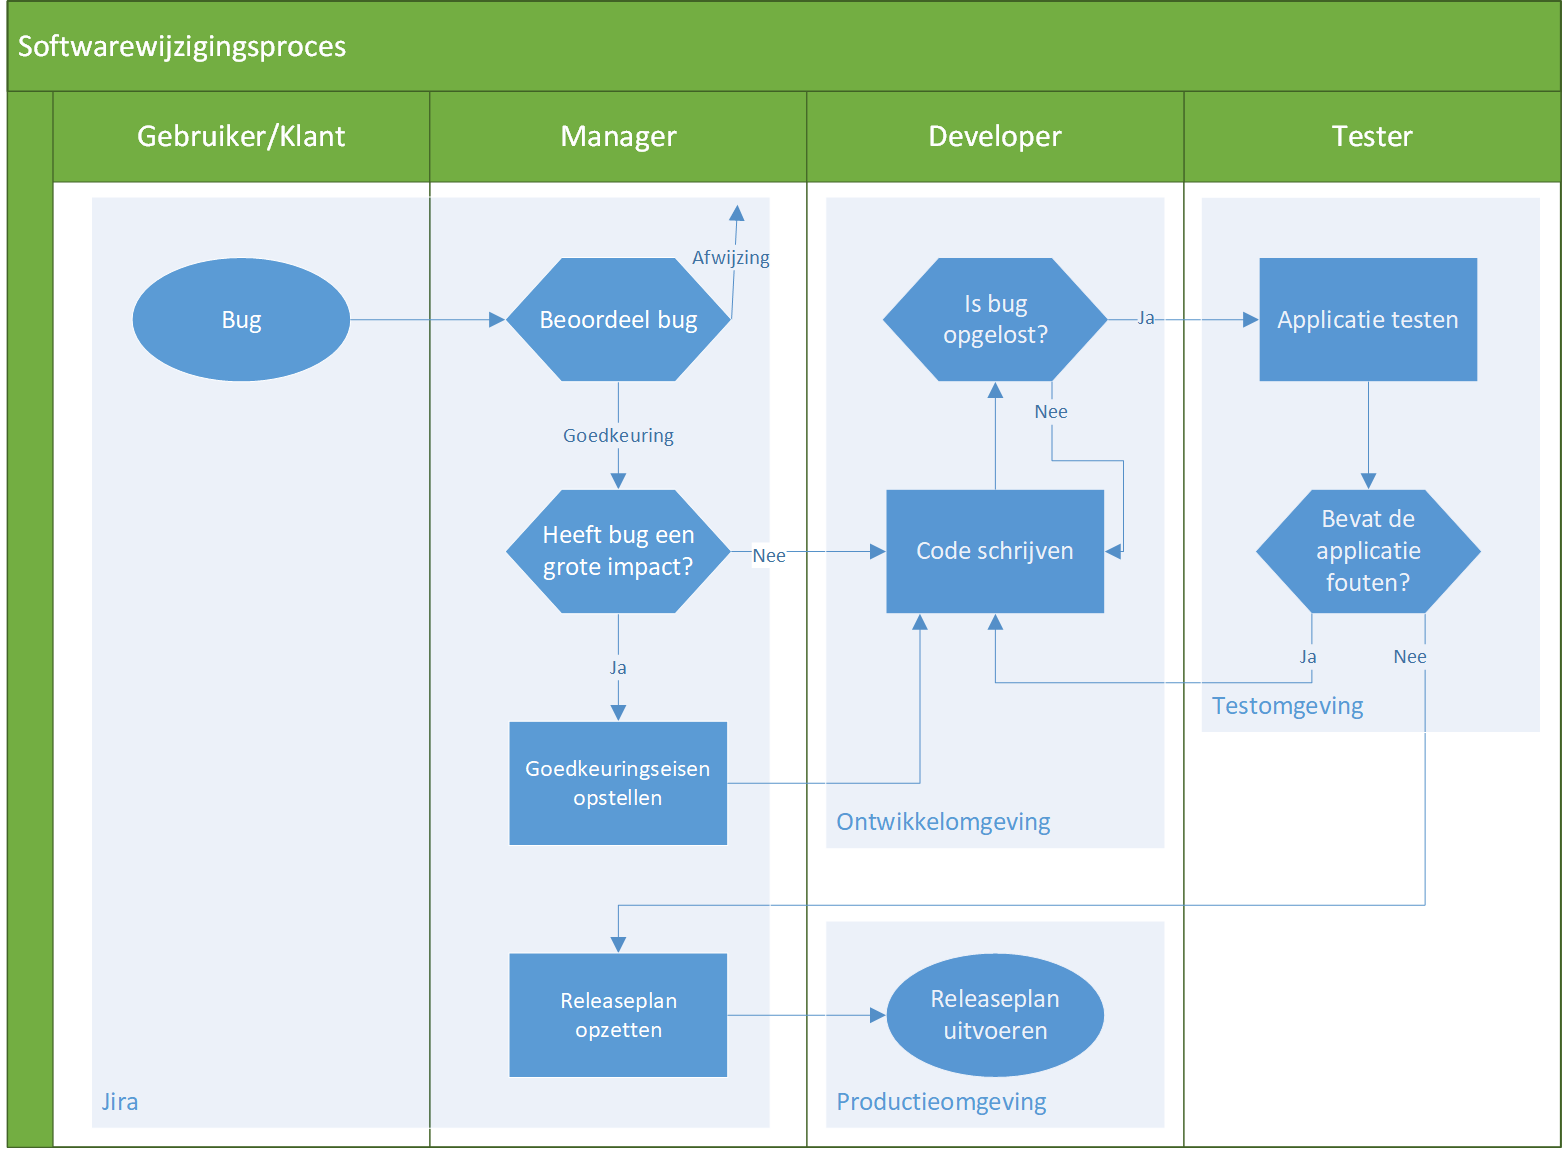
\includegraphics[width=\textwidth]{images/UMLActivityDiagram.png}
	\caption{Diagram van het softwarewijzigingsproces}
\end{figure}
Het proces begint bij de gebruiker/klant, welke een bug rapporteert in Jira. De manager beoordeelt vervolgens de bug, en zal deze goedkeuren of afkeuren. Als de bug goedgekeurd is wordt de bug nog beoordeeld op impact. Heeft de bug een grote impact, dan zal de manager goedkeuringseisen moeten opstellen. Dit is om te voorkomen dat de bug met grote impact bij de gebruiker terecht kan komen.

De bug komt nu bij de developer, die nu code gaat schrijven om de bug op te lossen. Hierna moet hij beoordelen of de bug opgelost is of niet. Dit beoordelen gebeurt op de ontwikkelomgeving en volgens een door de manager vastgestelde werkwijze. Zo is het mogelijk dat de manager bepaald dat de developer bij een webapplicatie de twee meestgebruikte browsers test. Als de bug nog niet is opgelost zal de developer opnieuw code moeten schrijven.

Nu de bug opgelost is in de ontwikkelomgeving is het de taak van de testers om de complete applicatie te testen op de testomgeving. De testers hebben een eigen werkwijze om de complete applicatie te testen, en hieruit zal blijken of de applicatie nog bugs bevat. Als dit zo is zal de developer de bugs moeten oplossen.

Als de applicatie door de testfase is gekomen zal de manager een releaseplan moeten opzetten. De developer zal dit plan vervolgens uitvoeren op de productieomgeving.

\end{document}